\begin{frame}{Generalizzazione}
Le classi con attributi comuni possono essere generalizzate.
    \begin{center}
        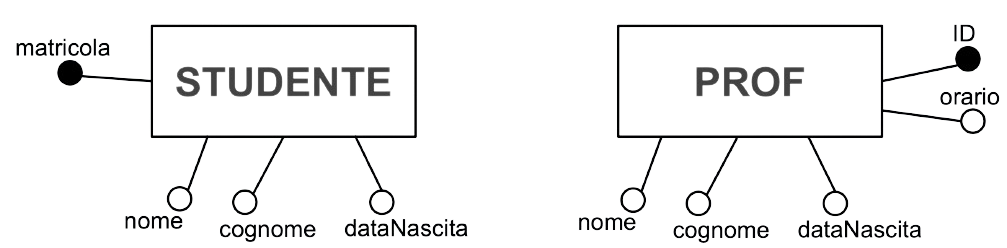
\includegraphics[width=.8\textwidth]{sections/er-model/img/generalization1.png}
    \end{center}
\end{frame}
%
\begin{frame}{Generalizzazione}
Le classi con attributi comuni possono essere generalizzate.
    \begin{center}
        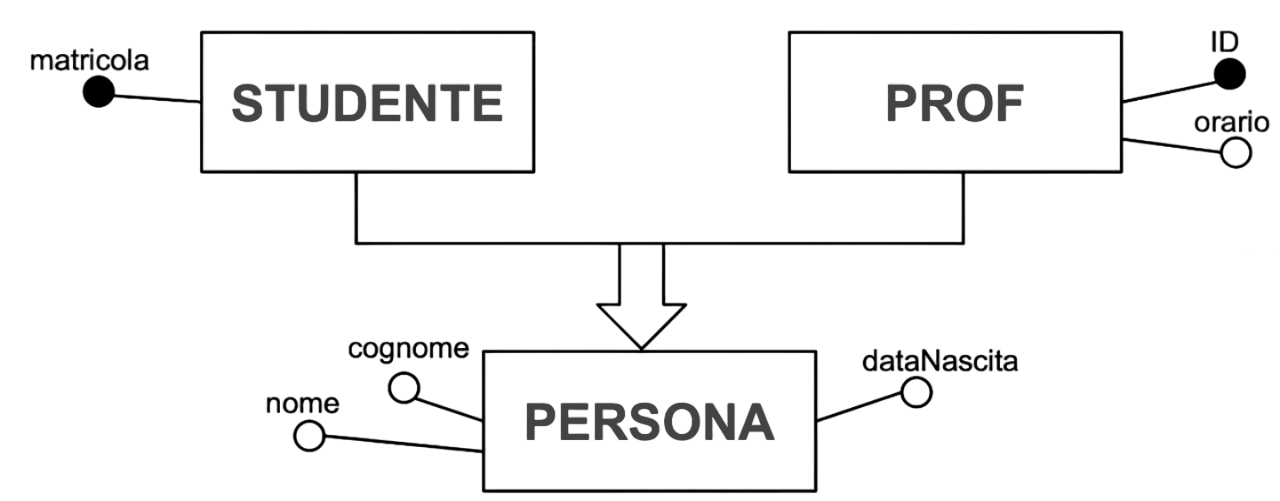
\includegraphics[width=.8\textwidth]{sections/er-model/img/generalization2.png}
    \end{center}
\end{frame}
%
\begin{frame}{Generalizzazione}
Altri simboli utilizzabili per i modelli E/R che a noi non interessano\ldots
    \begin{center}
        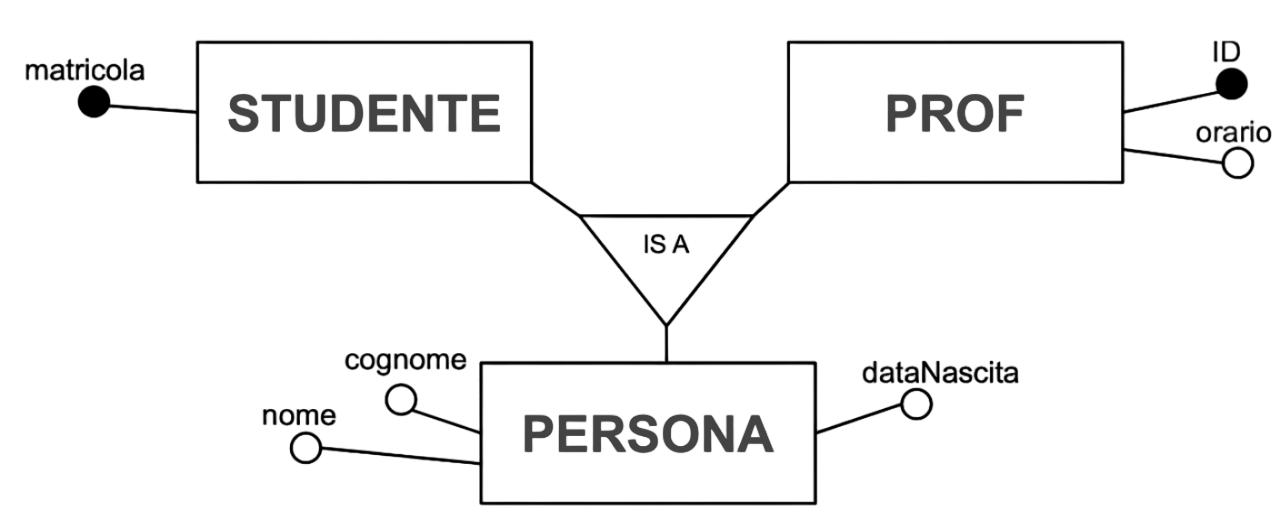
\includegraphics[width=.8\textwidth]{sections/er-model/img/generalization3.png}
    \end{center}
\end{frame}
%
\begin{frame}{Generalizzazione Parziale}
\begin{minipage}{.9\textwidth}
    \begin{block}{Generalizzazione Parziale}
        Una generalizzazione viene detta \textbf{parziale} se le specializzazioni non ricoprono tutti i casi possibili di una generalizzazione ma solamente alcuni.
    \end{block}
\end{minipage}
\begin{center}
    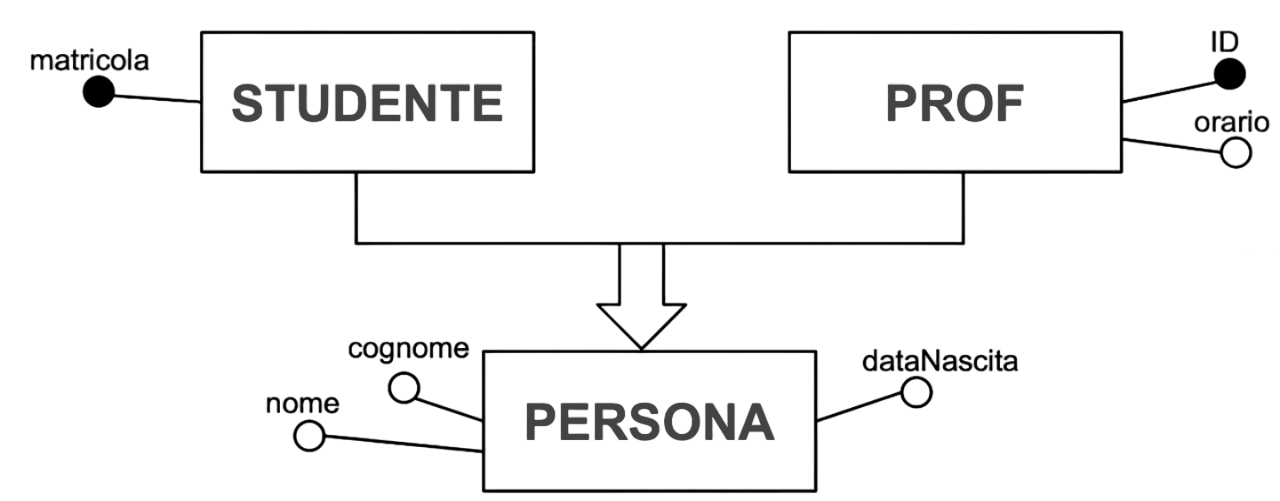
\includegraphics[width=.8\textwidth]{sections/er-model/img/generalization2.png}
\end{center}
\end{frame}
%
\begin{frame}{Generalizzazione Totale}
\begin{minipage}{.9\textwidth}
    \begin{block}{Generalizzazione Totale}
        Una generalizzazione viene detta \textbf{totale} se le specializzazioni ricoprono tutti i casi possibili di una generalizzazione.
    \end{block}
\end{minipage}
\begin{center}
    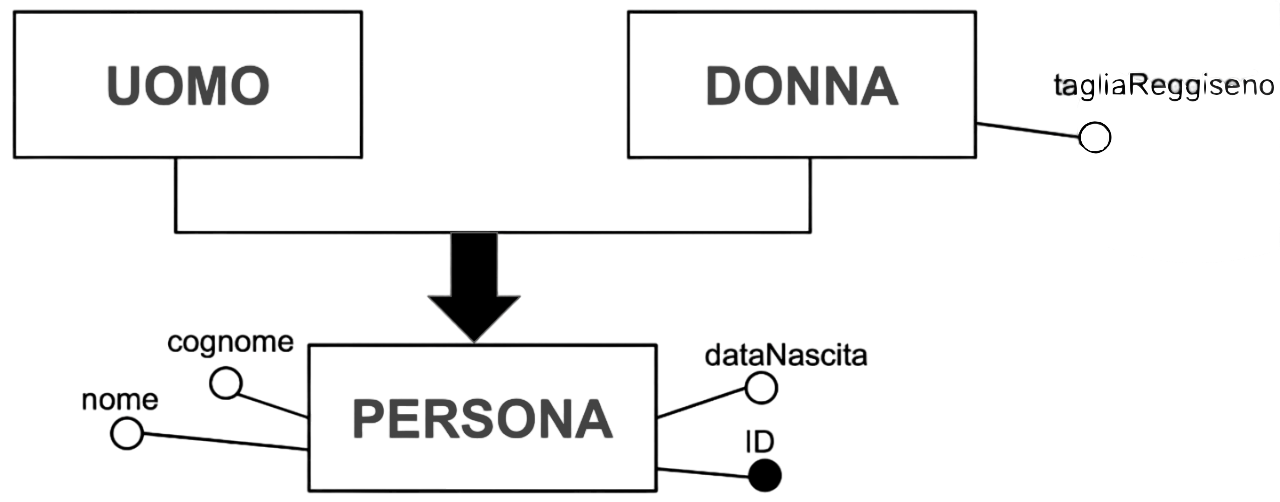
\includegraphics[width=.8\textwidth]{sections/er-model/img/generalization4.png}
\end{center}
\end{frame}
%
\begin{frame}{Generalizzazione Esclusiva}
\begin{minipage}{.9\textwidth}
    \begin{block}{Generalizzazione Esclusiva}
        Una generalizzazione viene detta \textbf{esclusiva} se le specializzazioni sono mutualmente esclusive.
    \end{block}
\end{minipage}
\begin{center}
    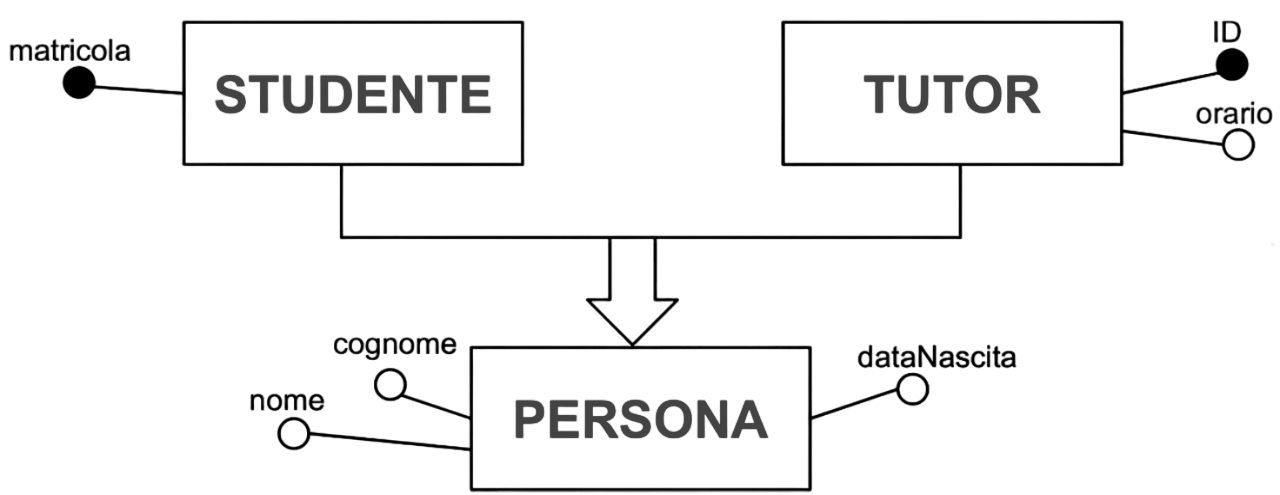
\includegraphics[width=.8\textwidth]{sections/er-model/img/generalization5.png}
\end{center}
\end{frame}
%
\begin{frame}{Generalizzazione}
Considerando tutte le combinazioni possibili delle propriet\`a appena viste possiamo avere 4 tipi di generalizzazione:
\begin{itemize}
    \item Totale Esclusiva (TE);
    \item Totale Sovrapposta (TS);
    \item Parziale Esclusiva (PE);
    \item Parziale Sovrapposta (PS).
\end{itemize}
\end{frame}